\section{Sieć końcowa}
\label{sec:final}

W rozdziale przedstawiono dokładność konfiguracji wybranej w strojeniu na zbiorze testowym dla pięciu ziaren oraz przebieg uczenia i błędy zgłoszonej sieci.

\subsection{Wyniki dla pięciu ziaren}
\label{sec:final-seeds}

Wyniki uczenia konfiguracji końcowej na pełnym zbiorze uczącym (podrozdział~\ref{sec:methodology-final}) przedstawiono w Tabeli~\ref{tab:final-seeds}. Średnia dokładność testowa wynosi \qty{97.91 +- 0.15}{\percent}, a wyniki pięciu ziaren mieszczą się w przedziale od \qty{97.74}{\percent} do \qty{98.12}{\percent}. Uczenie kończyło się po $8$ do $12$ epokach, a sieć zwracana przez wczesne zatrzymanie pochodziła z epoki od $3$ do $7$. Dokładność walidacyjna, \qty{97.79 +- 0.08}{\percent}, jest bliska testowej. W strojeniu ta sama konfiguracja osiągała na zbiorze walidacyjnym \qty{95.16 +- 0.39}{\percent} (Tabela~\ref{tab:tuning-summary}), ucząc się na \num{8000} zamiast \num{54000} obrazów.

\begin{table}[H]
    \centering
    \caption{Wyniki uczenia konfiguracji końcowej na pełnym zbiorze uczącym dla pięciu ziaren. Najlepsza epoka to epoka najmniejszej straty walidacyjnej, z której pochodzi sieć.}
    \label{tab:final-seeds}
    \begin{tabular}{lcccccc}
        \toprule
        Ziarno & Epoki & Najlepsza & \multicolumn{3}{c}{Dokładność [\%]} \\
        \cmidrule(lr){4-6}
        & & epoka & ucząca & walidacyjna & testowa \\
        \midrule
        1 & 10 & 5 & \num{99.34} & \num{97.73} & \num{97.74} \\
        2 & 12 & 7 & \num{99.64} & \num{97.90} & \num{98.12} \\
        3 & 8 & 3 & \num{98.96} & \num{97.83} & \num{97.95} \\
        4 & 9 & 4 & \num{99.29} & \num{97.70} & \num{97.80} \\
        5 & 10 & 5 & \num{99.44} & \num{97.78} & \num{97.92} \\
        \midrule
        średnia & \num{9.8} & \num{4.8} & \num{99.33 +- 0.25} & \num{97.79 +- 0.08} & \num{97.91 +- 0.15} \\
        \bottomrule
    \end{tabular}
\end{table}

\subsection{Zgłoszona sieć}
\label{sec:final-network}

Zgłoszona sieć to uczenie z ziarnem $1$, ustalonym przed uczeniem (podrozdział~\ref{sec:methodology-final}). Sieć \mbox{784-512-10} ma \num{407050} parametrów. Uczenie zakończyło się po $10$ epokach (\num{16880} iteracji), a wczesne zatrzymanie przywróciło sieć z epoki $5$. Jej dokładność testowa wynosi \qty{97.74}{\percent}, co odpowiada $226$ błędnie sklasyfikowanym obrazom spośród \num{10000}. Jest to najniższy wynik spośród pięciu ziaren z Tabeli~\ref{tab:final-seeds}.

Przebieg straty przedstawiono na Rysunku~\ref{fig:final-loss}. Strata ucząca maleje do epoki $8$, z \num{0.0201} w epoce $5$ do \num{0.0072}, a strata walidacyjna osiąga najmniejszą wartość, \num{0.08902}, w epoce $5$, a w kolejnych epokach waha się bez dalszego spadku. W epoce $8$ dokładność walidacyjna wynosiła \qty{98.05}{\percent}, ale strata walidacyjna, \num{0.08910}, była nieznacznie większa niż w epoce $5$. Ponieważ wczesne zatrzymanie kieruje się stratą, zwrócona sieć pochodzi z epoki $5$ i ma dokładność walidacyjną \qty{97.73}{\percent}.

\begin{figure}[H]
    \centering
    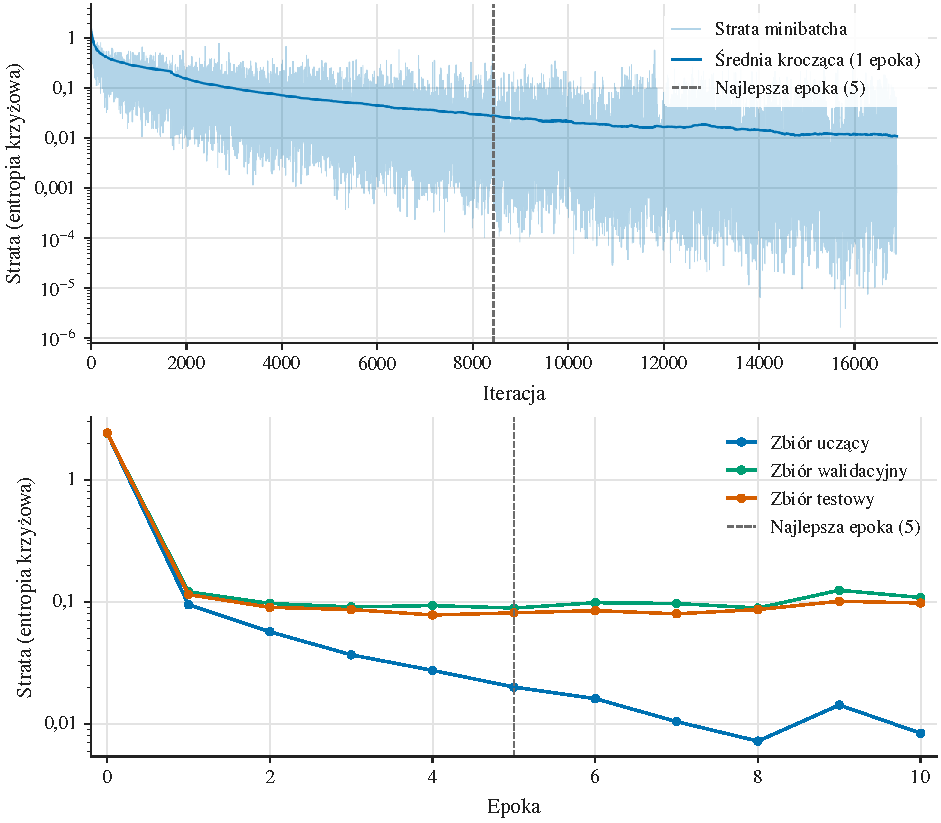
\includegraphics[width=0.9\textwidth]{mnist/final/plots/loss.pdf}
    \caption{Przebieg straty zgłoszonej sieci w skali logarytmicznej. Górny wykres: strata kolejnych paczek i jej średnia krocząca z okna jednej epoki. Dolny wykres: strata na zbiorach uczącym, walidacyjnym i testowym po każdej epoce. Linia przerywana oznacza epokę, z której pochodzi zwrócona sieć.}
    \label{fig:final-loss}
\end{figure}

Macierz pomyłek na zbiorze testowym przedstawiono na Rysunku~\ref{fig:final-confusion}. Najlepiej rozpoznawane są cyfry $0$ i $1$ (\qty{99.39}{\percent} i \qty{99.30}{\percent} poprawnych decyzji), a najsłabiej $4$ (\qty{94.30}{\percent}) i $8$ (\qty{95.69}{\percent}). Najczęstszą pomyłką jest klasyfikacja czwórki jako dziewiątki ($37$ obrazów, \qty{3.8}{\percent} czwórek). Kolejne pomyłki są co najmniej czterokrotnie rzadsze: ósemka jako $9$, $5$ i $3$ (po $9$ obrazów) oraz czwórka jako $7$ ($8$ obrazów).

\begin{figure}[H]
    \centering
    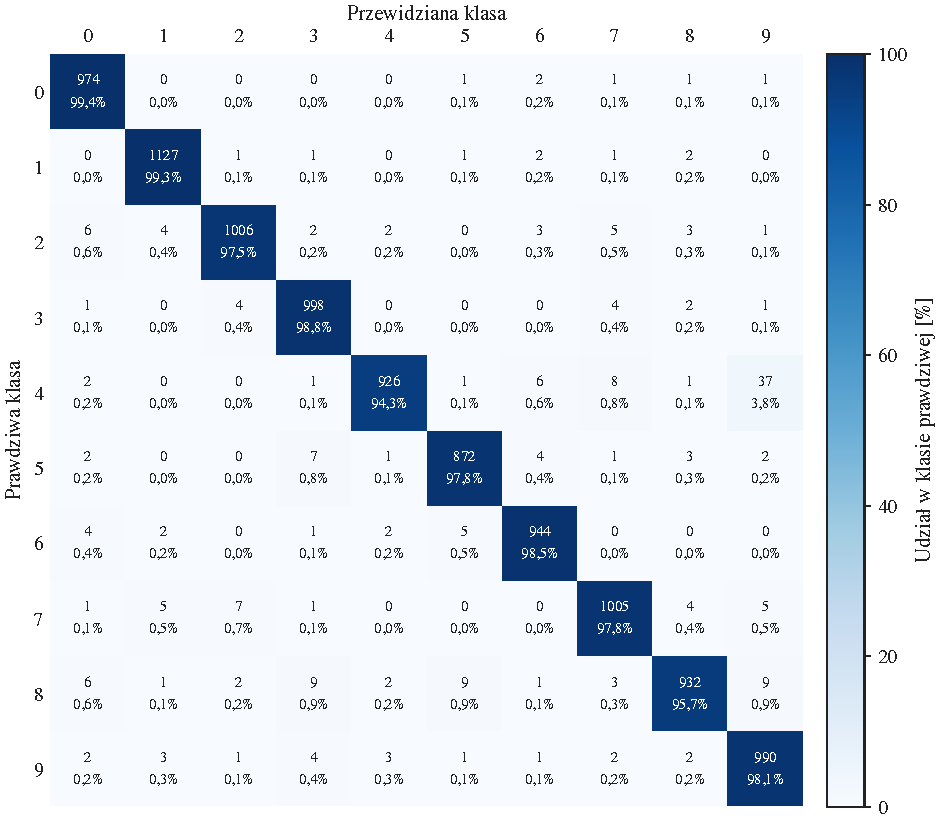
\includegraphics[width=0.75\textwidth]{mnist/final/plots/confusion_test.pdf}
    \caption{Macierz pomyłek zgłoszonej sieci na zbiorze testowym: liczba obrazów i odsetek w wierszu klasy prawdziwej.}
    \label{fig:final-confusion}
\end{figure}

Na Rysunku~\ref{fig:final-misclassified} pokazano $32$ błędnie sklasyfikowane obrazy testowe, którym sieć przypisała największe prawdopodobieństwo błędnej klasy. Spośród $226$ błędów $19$ ma prawdopodobieństwo przewidzianej klasy większe niż \num{0.99}, a $65$ większe niż \num{0.9}. Mediana tego prawdopodobieństwa wynosi dla błędów \num{0.77}. Wśród pokazanych obrazów są cyfry o nietypowym kształcie oraz cyfry przypominające przewidzianą klasę, np. czwórki z zamkniętą górną częścią sklasyfikowane jako $9$.

\begin{figure}[H]
    \centering
    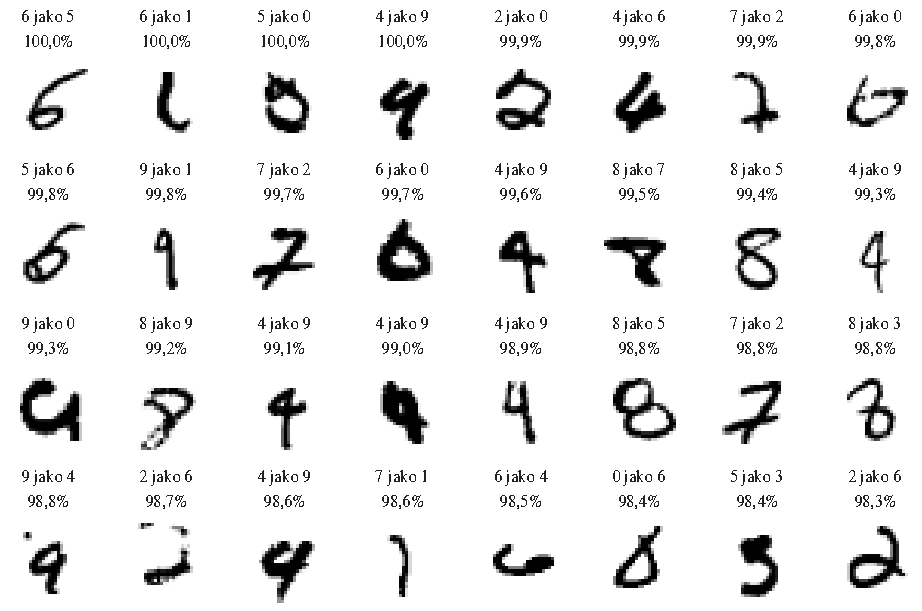
\includegraphics[width=\textwidth]{mnist/final/plots/misclassified.pdf}
    \caption{Błędnie sklasyfikowane obrazy testowe o największym prawdopodobieństwie przewidzianej klasy. Nad obrazem podano klasę prawdziwą, klasę przewidzianą i jej prawdopodobieństwo.}
    \label{fig:final-misclassified}
\end{figure}

Wagi łączące piksele obrazu z pierwszymi $32$ spośród $512$ neuronów warstwy ukrytej przedstawiono jako obrazy $28 \times 28$ na Rysunku~\ref{fig:final-weights}. Część neuronów ma wyraźne, lokalne skupiska wag o jednym znaku, układające się w fragmenty pociągnięć, a u pozostałych wagi nie tworzą widocznej struktury. Szarym kolorem oznaczono $72$ piksele, które mają wartość $0$ we wszystkich \num{54000} obrazach uczących. Zgodnie z podrozdziałem~\ref{sec:problem-dataset} ich wagi nie otrzymują gradientu i pozostają równe wartościom początkowym.

\begin{figure}[H]
    \centering
    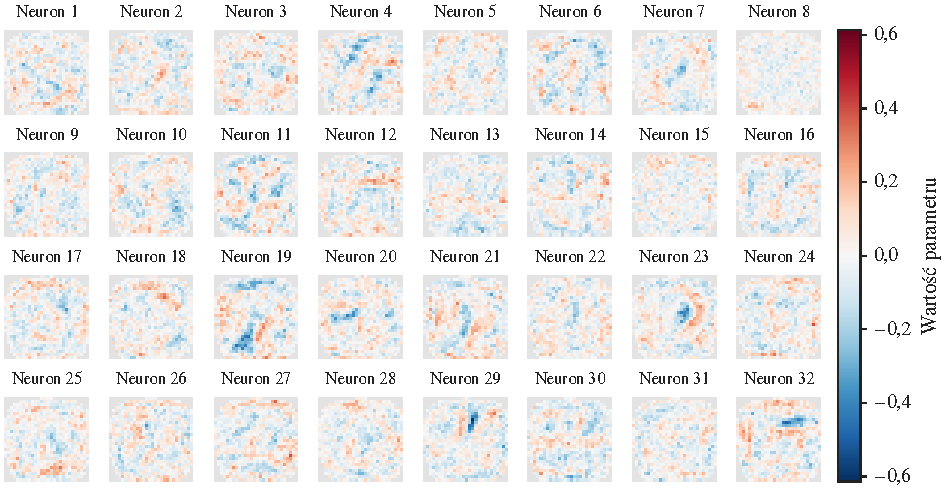
\includegraphics[width=\textwidth]{mnist/final/plots/first_layer_weights.pdf}
    \caption{Wagi pierwszej warstwy zgłoszonej sieci dla pierwszych $32$ neuronów warstwy ukrytej, przedstawione jako obrazy $28 \times 28$ we wspólnej skali barw. Szare piksele są stałe w części uczącej.}
    \label{fig:final-weights}
\end{figure}
